% !TeX root = ..\Proposta.tex

\vspace{2cm}

{ \Large \textbf{Resumo}}

\vspace{0.8cm}

{
\setstretch{1}

\noindent
A modelagem de chamas turbulentas de sprays diluídos geralmente é modelada utilizando modelos de evaporação e condensação, o que reproduz uma frente de chama externa às gotas.
No entanto, chamas envelopadas ao redor de gotas isoladas já foram observadas em experimentos e simulações de chamas turbulentas de sprays líquidos.
Também denominadas combustão de gotas isoladas, essas chamas já foram relacionadas ao processo de ignição de sprays e à formação de fuligem.
Revisando a literatura, constatou-se a necessidade de incluir a modelagem de chamas envelopadas em simulações turbulentas de sprays diluídos de combustíveis líquidos.
O desenvolvimento dessa modelagem deve representar efeitos de combustíveis reais, que são misturas de espécies químicas, como o querosene, e/ou hidrofílicos, como o etanol.
Para tanto devem incluir a capacidade de representação de uma mistura multicomponente, a consideração de fenômenos de transporte no interior da gota e a consideração de termodinâmica de mistura não ideal.
A construção de modelos de combustão de gota isolada (MCGI) passará pela construção de modelos de evaporação e condensação (MEC) com as mesmas funcionalidades, garantindo assim um aumento gradual da sofisticação dos modelos desenvolvidos e baseando-se sempre nos modelos já existentes na literatura.
A co-utilização de MEC e MCGI em uma simulação deve ser acompanhada por um mecanismo de seleção, também a ser desenvolvido, que escolherá qual modelo utilizar para cada gota.
Primeiramente, o novo modelo será testado de forma isolada, para garantir o correto funcionamento e implementação. 
Em seguida, será testado no cenário simplificado de uma chama laminar de névoa quiescente de spray líquido monodisperso.
Por fim, após aprofundamento em interação chama-turbulência, o modelo será utilizado em simulações multidimensionais turbulentas.

}
\vspace{1cm}

{ \Large \textbf{Abstract}}

\vspace{0.8cm}

{
\setstretch{1}

\noindent
The modeling of turbulent diluted spray flame is usually modelled using evaporation and condensation models, which produces an external flame sheet.
Nonetheless, enveloped flames around isolated droplets have already been seen in experiments and simulations of turbulent liquid spray flames.
Also named single or isolated droplet combustion, these flames have already been related to spray ignition processes and formation of soot.
Reviewing the literature, it was clear that the modeling of enveloped flames should be included in simulations of turbulent diluted liquid spray flames. 
The development of such models ought to represent real fuels which are mixtures of diferent chemical species, like kerosene, and/or hydrophilic, like ethanol.  
Therefore they must be able to represent multicomponent mixtures, to consider transport phenomena inside the droplet and to consider non-ideal mixture thermodynamics.
Developing single droplet combustion models (MCGI) will encompass the developement of evaporation and condensation models (MEC) with the same capabilities, thus ensuring a gradual model development process, which will be based on pre-existing models in the literature.
The simultaneous use of MEC and MCGi in a simulation must include a switch, also to be developed, that will chose which model to apply to each droplet.
The new model will first be tested independently, to ensure its correct working and implementation.
Then, it will be tested in the simplified cenario of a laminar flame in a quiescent monodisperse droplet mist.
Lastly, after investigating flame-turbulence interaction, the model will be used in multidimensionais turbulent spray flame simulations.

}\section{Introdução} \label{sec:intro}

A crescente demanda por transição energética e pela descarbonização da economia impulsiona a busca por alternativas aos combustíveis fósseis nos setores de energia, transporte, indústria. 
Alguns setores, como o energético e o de transportes urbano de baixa carga, têm apresentado avanço significativo na utilização de energias renováveis e na eletrificação, respectivamente \cite{MasriA2021}. 
Porém, combustíveis fósseis são extremamente difíceis de substituir em outros setores, especialmente os combustíveis líquidos.
Estes possuem maior energia específica e densidade energética \cite{Bergthorson2017,Julien2017}, assim adequados para aplicações de transporte, como no setor automotivo de cargas pesadas, naval e aeronáutico \cite{MasriA2021}.
Combustíveis líquidos são importantes também para algumas indústrias como aço e cimento, para algumas termoelétricas e até para máquinas de pequeno porte portáteis movidas a motor de combustão interna (MCI).
Soma-se a isso uma análise histórica que indica que a transição para fontes renováveis se dará ao longo de décadas \cite{MasriA2021}.

Nota-se que processos de combustão continuarão relevantes nas próximas décadas.
Em especial, todas as aplicações mencionadas baseiam-se na combustão turbulenta de sprays líquidos.
Assim, é necessário buscar soluções que conciliem essa tecnologia com os esforços de transição energética e descarbonização da economia.
A comunidade científica busca, então, três caminhos: \textbf{(i)} desenvolver tecnologias para novos combustíveis (como  etanol, metanol, hidrogênio e amônia \cite{FAPESP_etanol_1,VerhelstS2019,TeohY2023,ElbazA2022}); \textbf{(ii)} desenvolver novas origens para os mesmos combustíveis (como SAF, biocombustíveis e eletro-combustíveis \cite{BenJames-SAF,BergthorsonJ2015,WestbrookC2019,PalysM2022}); \textbf{(iii)} melhorar a eficiência dos motores a combustão e reduzir a formação de poluentes \cite{MasriA2021}.

Independente da origem do combustível, o processo de combustão deve ser compreendido para que motores e queimadores eficientes e com baixa emissão de poluentes sejam desenvolvidos.
Para tanto é necessário pesquisa em combustão, que pode ser estruturada em trabalhos experimentais e trabalhos de modelagem.
A modelagem da combustão turbulenta de sprays, foco dessa proposta, deve ser capaz de contemplar diferentes combustíveis líquidos, incluindo combustíveis oriundos das demandas (i) e (ii).
Deve também representar os diferentes fenômenos envolvidos nesse processo, como ignição e formação de poluentes, para atender a demanda (iii).
No âmbito da combustão turbulenta de sprays, é de extrema importância o modelo de transferência de calor e massa da gota (líquida) para a fase gasosa (HMT -\emph{Heat and Mass Transfer}).
Modelos HMT regem, dentre outros aspectos, a taxa de vaporização do combustível das gotas do spray.
É conhecido que essa modelagem tem enorme influência na chama \cite{JennyB2012}, influenciando a sua estrutura, temperatura, geometria e formação de poluentes.


Nesse sentido, revisando a literatura mais recente, nota-se a necessidade de maior desenvolvimento de \textbf{modelos de evaporação e condensação} (MEC) para representar corretamente diferentes combustíveis.
Por exemplo, modelos monocomponentes com equilíbrio termodinâmico não são capazes de representar todos os fenômenos associados, por exemplo, à combustão de etanol \cite{SacomanoF2024CF}, combustível de importância estratégica para o Brasil e para a Índia \cite{etanol-BNDES,etanol-India}.
Em especial, nota-se uma demanda pela aplicação de modelos sofisticados, desenvolvidos e testados na escala de uma única gota ou em simulações
laminares ou unidimensionais, em simulações multidimensionais de combustão turbulenta.
Para representar combustíveis reais como o etanol é necessário modelar a gota com abordagem de substância \textbf{multicomponente}, considerando \textbf{termodinâmica de mistura não-ideal} e os efeitos de transferência de calor e massa no \textbf{interior da gota}.

Em MECs, a evaporação da gota fornece vapor de combustível que alimenta a chama.
Nessa abordagem, a chama não é estabilizada por uma gota em específica, mas se estabilizada por fenômenos específicos ao escoamento gasoso \cite{ChiuH1982,Law2006}.
Esse modo de combustão de spray é chamado \textbf{combustão com frente de chama externa}, ou simplesmente \textbf{combustão externa}.
Em contraste, é possível que as gotas entrem em combustão individualmente, com a evaporação de combustível alimentando uma frente de chama próxima e envolvente a cada gota, a uma distância na mesma ordem de grandeza que o diâmetro da gota \cite{ChiuH1977}.
Isso é chamado \textbf{combustão de gota isolada}.

Experimentos indicam que a combustão de gota isolada ocorre tanto durante a ignição	de sprays \cite{AggarwalS2014} quanto em sprays já desenvolvidos \cite{ChenG1996CF,SinghG2020,GounderJ2009PhD}.
Simulações DNS (\emph{Direct Numerical Simulation}) e LES (\emph{Large Eddy Simulation}) também indicam a ocorrência de combustão de gota isolada nessas duas etapas da combustão turbulentas de sprays líquidos (\cite{BorghesiG2013CF} e \cite{PaulhiacD2020,BojkoDesJardin2017CF}, respectivamente).
A combustão de gota isolada também ocorre na combustão de alguns pós metálicos que queimam em combustão homogênea na fase gasosa, como o alumínio \cite{Bergthorson2015,Julien2017,Baumann2020}, segundo várias evidências experimentais \cite{Braconnier2020Pre,Braconnier2022,Bucher1999,Halter2023}.
A Figura \ref{fig:sdc-exp} mostra evidências da combustão de gota isolada em sprays turbulentos de etanol (Figuras \ref{fig:GounderJ2009-7.17} e \ref{fig:SinghG2020-10}) e na combustão de uma partícula alumínio (Figura \ref{fig:Braconnier202PhD-5.20}). %\todo{explicar figuras ...}

Além disso, alguns trabalhos apontam para a combustão de gota isolada em sprays líquidos como uma fonte de emissão de fuligem \cite[e referências 3-13 \emph{loc. cit.}]{FachiniF2005}, de forma que a modelagem desse fenômeno contribui com os esforços de limitar as emissões desse poluente.

\begin{figure}[H]
    \centering
    \caption{Observações experimentais de combustão de gota isolada em chamas de etanol na Fig. \ref{fig:GounderJ2009-7.17} e \ref{fig:SinghG2020-10}, indicadas por setas, e ao redor de uma partícula de pó de alumínio na Fig. \ref{fig:Braconnier202PhD-5.20}. 
    Siglas: LIF -- \emph{Laser Induced Fluorescence}; HR -- \emph{Heat Release}.
    Adaptadas de \cite{GounderJ2009PhD,SinghG2020,Braconnier2020Pre}.
    }
    \begin{subfigure}[t]{0.39\textwidth}
        \centering
        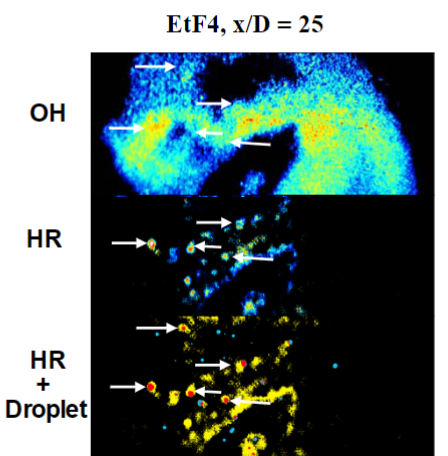
\includegraphics[width=0.99\textwidth]{30_images/GounderJ2009-7.17-1.png}
        \caption{LIF de OH, HR e HR sobreposto com posição das gotas em uma chama de etanol no queimador \emph{Sydney piloted spray burner}, 25 diâmetros do injetor a jusante. Adaptado de \cite[Fig. 7.13]{GounderJ2009PhD}.}
        \label{fig:GounderJ2009-7.17}
    \end{subfigure}
    \hfill
    \begin{subfigure}[t]{0.59\textwidth}
        \centering
        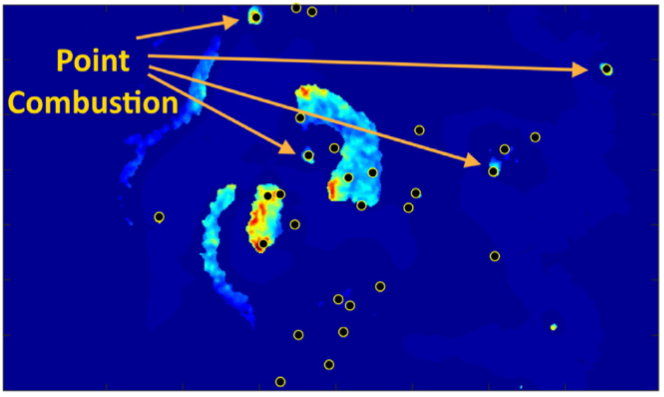
\includegraphics[width=0.99\textwidth]{30_images/SinghG2020-10.png}
        \vfill
        \caption{HR sobreposto com posição das gotas em uma chama de etanol no queimador \emph{Sydney piloted needle spray burner}, 20 diâmetros do injetor a jusante. Adaptado de \cite[Fig. 10]{SinghG2020}.}
        \label{fig:SinghG2020-10}
    \end{subfigure}
    \vspace{0.5cm}
    \begin{subfigure}[b]{0.8\textwidth}
        \centering
        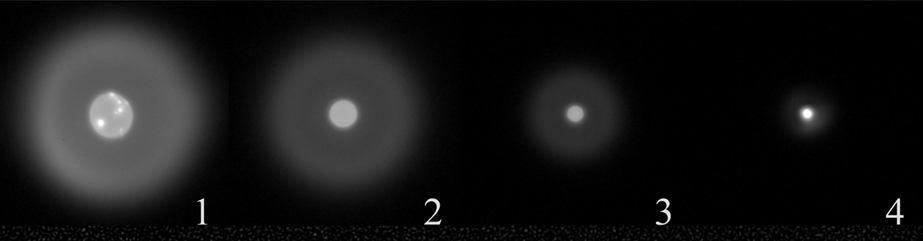
\includegraphics[width=0.99\textwidth]{30_images/Braconnier202PhD-5.20.png}
        \caption{Fotografias de combustão de uma partícula de alumínio de $\qntdd{50}{\mu m}$ de diâmetro em atmosfera 80\% Argônio/ 20\% oxigênio. Adaptado de \cite[Fig. 5.21]{Braconnier2022}.}
        \label{fig:Braconnier202PhD-5.20}
    \end{subfigure}
    \label{fig:sdc-exp}
\end{figure}

Assim, constata-se que modelar a combustão de gota isolada é importante para a ignição de sprays de combustíveis líquidos, para a emissão de poluentes (em particular de fuligem) e também para a combustão de alguns combustíveis metálicos. 
Revisando a literatura, constatou-se a necessidade de desenvolver modelos de combustão de gota isolada (MCGI) capazes de representar corretamente diferentes combustíveis, incluindo as mesmas capacidades mencionadas para os MECs.
Notou-se também que não é claro na literatura quando a combustão de gota isolada ocorre \cite[p. 8]{JennyB2012} -- apesar de existirem diferentes modelos em cenários simplificados, a serem discutidos -- nem a influência de modelar a combustão de gota isolada (MCGIs) junto com a combustão externa (representada por MECs) na combustão turbulenta multidimensional.


\subsection{Objetivos} \label{sec:objetivos}

Tendo em vista os aspectos levantado anteriormente, a tese proposta tem como objetivo o \yellow{desenvolvimento de estratégias para a simulação da transferência de calor e massa} em gotas em dois cenários: (\textbf{A.}) combustão externa; (\textbf{B}.) combustão de gota isolada.
Esses cenários correspondem aos seguintes modelos HMT:
\begin{enumerate}
    \item[\textbf{A.}] Modelo de Evaporação e Condensação (MEC); e 
    \item[\textbf{B.}] Modelo de Combustão de Gota Isolada (MCDI).
\end{enumerate}
Esses modelos devem considerar os seguintes aspectos: 
\begin{enumerate}
    \item[\textbf{1.}] Descrição multicomponente da gota; 
    \item[\textbf{2.}] Gota com termodinâmica de mistura não-ideal; 
    \item[\textbf{3.}] Consideração dos efeitos de transferência	de calor e massa no interior da gota. 
\end{enumerate}
O objetivo é desenvolver aplicar a estratégia desenvolvida em simulações turbulentas reativas multidimensionais, com ambos modelos, {A} e {B} e com a funcionalidade:
\begin{enumerate}
    \item[\textbf{4.}] Determinação de quando ocorre a combustão de gota isolada;
\end{enumerate}
ou seja, de determinar se a gota se encontra no cenário {A} ou {B} e escolher o modelo apropriado para a correta representação dos fenômenos envolvidos.
Visando a aplicação em simulações CFD (\emph{Computational Fluid Dynamics}) turbulentas, reativas e multidimensionais, as estratégias a serem desenvolvidas devem ser robustas e computacionalmente eficientes.

O modelo HMT de simulações CFD que utilize as estratégias a serem desenvolvidas, incluindo as funcionalidades {1}, {2}, {3} e {4}, terá maior complexidade teórica em comparação aos modelos utilizados pela literatura. 
Isso permitirá ao autor dessa proposta investigar o efeito de considerar a combustão de gota isolada, e dos aspectos {1}, {2} e {3}, na estrutura da chama.
A investigação da estrutura da chama inclui a investigação de aspectos como distribuição de temperatura e concentrações de espécies, o que é essencial para a determinação da ignição, da eficiência de combustão e das emissões de poluentes.
A relação da estratégia a ser desenvolvida \yellow{com a emissão de poluentes e com a ignição de sprays também será investigada.}% !TEX root = ../Proposta.tex


\section{Fundamentação Teórica}


\subsection{Combustão Turbulenta de Sprays} \label{sec:teoria}

A combustão turbulenta de sprays é caracterizada pela competição de vários processos físicos e químicos, fortemente acoplados e em diferentes escalas de tempo e comprimento. 
Na formação de um spray turbulento, um jato de combustível líquido se quebra devido às instabilidades hidrodinâmicas de Kevin-Helmholz e Rayleigh-Taylor, formando gotas que se dispersam, eventualmente se deformam e rompem, quando as forças aerodinâmicas superam as tensões superficiais da gota, formando novas gotas \cite{JennyB2012}.
Isso forma o \textbf{regime denso} do spray, onde ocorrem também outros fenômenos como colisões, coalescência e interferência por esteira aerodinâmica, por turbulência ou por alteração da concentração de vapor de combustível devido à evaporação.
A medida que o jato se atomiza em gotas menores e dispersas, as gotas deixam de interferir umas nas outras e o regime é chamado de \textbf{disperso} ou \textbf{diluído}. 
Desde a sua formação, as gotas de combustível evaporam, fornecendo vapor combustível para a chama, que por sua vez influencia e é influenciada pelas próprias gotas e pela turbulência local.
Revisões detalhadas e com mais referências para processos e interações subjacentes à combustão turbulenta de sprays podem ser encontradas em \cite{JennyB2012, MasriA2016, SanchezA2015, ZhouL2021,JiangX2010}.

O foco deste trabalho é na modelagem das escalas da gota (escala micro), que será utilizada em simulações CFD turbulentas multidimensionais, na escala do spray e da chama (escala macro), considerando apenas a região diluída de sprays de combustível líquido.
Simulações CFD multidimensionais de chamas turbulentas de spray requerem, dentre outras, a modelagem da fase contínua, gasosa, da combustão turbulenta e da fase dispersa, as gotas.
A modelagem da fase gasosa é discutida na Seção \ref{sec:gas}, seguida pela modelagem da combustão turbulenta de sprays na Seção \ref{sec:comb-sprays}. 
Por fim, a modelagem da fase discreta é apresentada na Seção \ref{sec:gotas}.
Os modelos de gota, escala micro, são discutidos nas seções seguintes: MEC na Seção	\ref{sec:MEC} e MCGIS na Seção \ref{sec:MCGI}.


\subsubsection{Modelagem da Fase Contínua} \label{sec:gas}

Neste trabalho, será empregada a abordagem Euler-Lagrange, na qual a fase gasosa é tratada como contínua (descrição euleriana) e as gotas líquidas são representadas como partículas pontuais (descrição lagrangiana), cuja trajetória e evolução são acompanhadas ao longo da simulação. 
As equações de transporte da fase contínua — conservação de espécie química, quantidade de movimento e energia — são discretizadas no tempo e no espaço, em aplicações CFD, geralmente seguindo o Método dos Volumes Finitos \cite{Anderson2009}.
A consideração das gotas como partículas pontuais faz-se necessária devido à grande diferença de escalas de comprimento entre as gotas e o spray e à alta densidade de gotas no spray.
Nessa técnica, conhecida como \emph{Particle Source In Cell} (PSIC), a interação entre as gotas e o escoamento é representada por termos fonte nas células do domínio computacional, o que permite contabilizar os efeitos acumulados das partículas sobre a fase contínua de maneira robusta e eficiente para simulações de chama turbulenta tridimensionais.

A modelagem da fase gasosa em simulações CFD turbulentas requer um tratamento para descrever a turbulência. 
Nesse sentido, as simulações das grandes escalas (método LES) tem se mostrado uma boa ferramenta para a combustão turbulenta de sprays \cite{SacomanoF2020CF}, especialmente devido a capacidade de simular fenômenos intrinsicamente transitórios como turbulência e processos spray.
A simulação de chamas turbulentas de spray com LES, junto com o método de interação chama-turbulência ATF (\emph{Artificially Thickened Flame}), a ser explicado, vem sendo desenvolvida pelo grupo de pesquisa \cite{SacomanoF2017PhD,SacomanoF2019Fluids,SacomanoF2017CF,SacomanoF2020CF,SacomanoF2018CTM}.

Nessa abordagem, as variáveis transportadas são espacialmente filtradas de acordo com $\psi = \widetilde\psi + \psi^"$ usando um filtro de comprimento $\Delta_{malha}$. $\psi^"$ são as flutuações sub-escala (SGS - \emph{sub-grid scale}) e $\widetilde\psi$ representa a quantidade filtrada espacialmente, ponderada pela massa específica, $\widetilde\psi = \overline{\rho\psi}/\overline\rho$.
Utilizando uma formulação de densidade variável para baixos números de Mach, as equações de transporte de massa e de quantidade de movimento são
\begin{equation}
    \frac{\partial \overline \rho}{\partial t} + 
    \frac{\partial \overline \rho \widetilde u_j}{\partial x_j} = 
    \overline S_m,
\end{equation}
\begin{equation}
    \frac{\partial \overline\rho \widetilde u_i}{\partial t} + 
    \frac{\partial \overline\rho \widetilde u_i \widetilde u_j}{\partial x_j} =
    \frac{\partial }{\partial x_j} \left(
        2\overline\mu \widetilde S_{ij} -
        \frac{2}{3}\overline\mu \frac{\partial \widetilde u_k}{\partial x_k} \delta_{ij} -
        \overline\rho \tau_{ij}^{\text{sgs}}
    \right) -
    \frac{\partial \overline p}{\partial x_i} +
    \overline p g_i + 
    \overline S_{u,i}.
\end{equation}
Na equação de transporte de massa da mistura, $\rho$ é a massa específica da mistura, $t$ é o tempo, $u_j$ os componentes da velocidade na direção $j$ ($j=1,2,3$).
Na equação de transporte de quantidade de movimento, $\mu$ é a viscosidade dinâmica, $S_{ij}$ é o tensor da taxa de deformação, $\delta_{i,j}$ é o delta de Kronecker, $p$ é a pressão e $g_i$ é o componente da aceleração da gravidade na direção	$i$ ($i=1,2,3$). 
Os termos de acoplamento entre fases devido à presença da fase dispersa, $S_m$ e $S_{u,i}$,  são termos fontes de massa e de quantidade de movimento, respectivamente.
É através desses termos que os efeitos das gotas, calculados usando os modelos de gota, são considerados na fase gasosa.
$\tau_{ij}^{sgs}$ é o tensor das tensões originados pelos termos sub-malha.
Nos trabalhos do grupo de pesquisa, os termos de acoplamento entre fase seguem a implementação de Chrigui\etal{} \cite{ChriguiM2012} e o tensor SGS é fechado utilizando o modelo de Smagorinski \cite{Pope2000} com o procedimento dinâmico de Germano\etal \cite{Germano1991}.


\subsubsection{Modelagem da Combustão Turbulenta de Sprays} \label{sec:comb-sprays}

No contexto de combustão externa, com o uso de MECs, entende-se que a chama formada é uma chama pré-misturada, devido ao vapor de combustível evaporado pelas gotas se misturar com o oxidante do ambiente \cite{PoinsotVeynante2005}.
Em simulações de combustão nas grandes escalas, a frente de chama pertence a escala sub-malha.
Ademais, o aspecto não linear dos termos de reação faz com que a frente de chama não seja corretamente representada pelas quantidades filtradas \cite{SacomanoF2017PhD}.
Assim, a modelagem de combustão turbulenta de sprays requer um tratamento matemático para essa interação.
Existem diferentes abordagens para modelar com a interação chama-turbulência, que podem ser classificadas em abordagens estocásticas (baseadas em funções de distribuição de probabilidade) e abordagens determinísticas.

Dentre as abordagens determinísticas, se destaca o espessamento artificial da chama (ATF), que vem sendo utilizado pelo grupo de pesquisa.
O ATF aborda a interação chama-turbulência de duas maneiras: o espessamento artificial da chama e o amarrotamento da frente de chama causado pela turbulência.
O espessamento artificial da chama traz o efeito da interação chama-turbulência para as grandes escalas, permitindo que a resolução da chama em células típicas de LES.
O amarrotamento da frente de chama, no contexto do ATF, é considerado por uma função de eficiência que acelera a velocidade da frente de chama.
O efeito do espessamento artificial e do amarrotamento de chama se manifestam na equação de transporte de um escalar $\psi$ através dos fatores de espessamento $F$ e da função de eficiência $E$.
A equação de transporte para os escalares  $\psi=\lbrace h, Z\rbrace$, ou seja, para a energia (na forma da entalpia total) e para a fração da mistura, tem a forma, em uma formulação de densidade variável para baixos números de Mach,
\begin{equation}
    \frac{\partial \bar \rho \widetilde \psi}{\partial t} + 
    \frac{\partial \bar \rho \widetilde \psi \overline u_j}{\partial x_j} =
    \frac{\partial }{\partial x_j} \left[ \left(
    FE^*_\Delta \frac{\bar\mu}{\text{Sc}_\psi} + (1-\Omega)\frac{\mu_t}{\text{Sc}_{t,\psi}}
    \right) \frac{\partial \widetilde \psi}{\partial x_j}
    \right] +
    \frac{E^*_\Delta}{F}\widetilde{\dot{\omega}_\psi} + 
    \overline S_{\psi,\nu}.
    \label{eq:FGM}
\end{equation}
A entalpia da mistura é dada por $Z=Y_f/{(Y_f+Y_{ox})}$, sendo $Y_f$ a fração mássica do combustível e $Y_{ox}$ a fração mássica do oxidante.
$\text{Sc}_{\psi}$ e $\text{Sc}_{\psi,t}$ são os números de Schmidt laminar e turbulento.
% $\Omega$ é o sensor da chama e $\dot \omega_\psi$ é a taxa de reação. 
$S_{\psi,\nu}$ é o termo de acoplamento entre as fases representando a fonte de vapor oriunda da fase dispersa, sendo não nulo apenas na equação da fração de mistura, i.e. quando $\psi=Z$.

$\Omega$ é o sensor da chama, que permite aplicar o espessamento apenas nas regiões onde a chama está presente (\emph{espessamento dinâmico}).
Nos trabalhos do grupo de pesquisa do candidato, o LETE (Laboratório de Engenharia Térmica e Ambiental), utiliza-se o fator de espessamento $F$ variável de acordo com as propriedades da mistura $Z$ e $h$ e com o tamanho da malha \cite{SacomanoF2017PhD,SacomanoF2017CF}.
A função de eficiência $E$ baseia-se na função de potência de Charlette \cite{CharletteF2002}, cujo com expoente $\beta$ pode ser assumido constante (como em \cite{SacomanoF2017PhD,SacomanoF2017CF,SacomanoF2019IJHMT,ShastryV2023,SekularacN2024}) ou variável de acordo com as propriedades da mistura (como em \cite{SacomanoF2020CF}).

No contexto do trabalho do grupo de pesquisa, a taxa de reação $\dot \omega_\psi$ vem do método de química pré-tabelada chamado \emph{Flamelet Generated Manifold} (FGM).
Nessa abordagem, os estados termoquímicos da mistura são calculados antecipadamente, mapeados e salvos, para serem acessados por variáveis de acesso transportadas durante a simulação.
Nos trabalhos do grupo de pesquisa, as tabelas químicas são geradas por simulações de chamas livres, unidimensionais, laminares e pré-mixadas, os chamados \emph{flamelets}.
Dessa forma, duas variáveis de acesso são suficientes: a fração de mistura $Z$ e uma variável de progresso da reação $Y_{pv}$, definida como uma combinação linear de frações mássicas de algumas espécies e suas massas molares \cite{SacomanoF2018CTM}.    
    

\subsubsection{Modelagem Da Fase Discreta} \label{sec:gotas}

A evolução das gotas na abordagem Euler-Lagrange com aproximação de gotas pontuais é regida por equações diferenciais ordinárias (EDOs) no tempo para taxa de variação da posição, velocidade, massa e temperatura da gota.

Considere uma única gota dentro do spray, composta por $k=1,\ldots,n-1$ espécies (componentes).
O subscrito $d$ se refere à gota (\emph{droplet} em inglês).
Sua posição é dada pelas coordenadas do seu centro de massa $X_{d,i}$, $i=1,2,3$, sua velocidade por $U_{d,i}$ nas direções $i$, sua massa por 
\begin{equation}    
    m_d = \sum_{i=1}^{n-1} m_{i}^k
\end{equation}
e sua temperatura por $T_d$, assumida uniforme em seu interior (hipótese de \emph{condutividade térmica infinita}).
A evolução da gota $k$ é então regida pelas EDOs \cite{JennyB2012}
\begin{gather}
    \frac{\diff X_{d,i}}{\diff t} = U_{d,i}
    \label{eq:Ud}\\
    \frac{\diff U_{d,i}}{\diff t} =
    \frac{f_i}{ m_{d}} -
    g_i 
    \label{eq:Xd} \\
    \frac{\diff m_{d}}{\diff t} = \sum_{k=1}^{n-1} \dot m_{d,k}
    \label{eq:md} \\
    % \frac{\diff h^{k}_i}{\diff t} = \dot h^{k}_i
    m_d \sum_{k=1}^{n-1} Y_{L,k} c_{L,k} \frac{\diff T_d}{\diff t} = \dot q_d
    \label{eq:Td}
\end{gather}
em que $f_i$ representa os componentes das forças resultantes da fase gasosa na gota, $g$
$\dot m_{d,k}$ é a taxa de variação de massa da espécie $k$ na gota e $\dot q_d$ o a taxa líquida de transferência de calor para a gota.
$ m_d \sum_k Y_{L,k} c_{L,k}$ é a capacidade térmica da gota, em que 
$Y_{L,k}$ e $c_{L,k}$ são a fração mássica e o calor específico da  espécie $i$ na fase líquida.
Os termos $f_i$, $\dot m_{d,k}$ e $\dot q_d$ são termos de acoplamento entre as fases na escala da gota, ou seja, representam a interação entre as fases líquida e gasosa na interface da gota.
Enquanto o primeiro termo é geralmente substituído por uma expressão semiempírica para o arrasto e o segundo por um termo de flutuação (\emph{vd.} \cite[p. 16]{JennyB2012}), os dois últimos precisam de um modelo HMT.
O modelo HMT pode descrever a combustão externa, no caso de um MEC, ou a combustão de gota isolada, no caso de um MCGI.  



\subsection{Modelos de Evaporação e Condensação (MEC)} \label{sec:MEC}

Na escala de uma gota, o problema pode ser dividido em duas regiões segregadas: a gota, líquida; e o gás ambiente circundante. 
Cada região é governada por um conjunto de equações.
Ambas regiões podem ser simuladas numericamente ou representadas por um modelo simplificado, com diferentes níveis de descrição.
Trabalhos que simulam numericamente tanto o interior quanto o exterior da gota são capazes de simular muitos efeitos físicos a um elevado custo computacional.
Esses modelos são chamados de modelos resolvidos, detalhados ou até de computações, pois as equações de transporte foram resolvidas em detalhes nas duas regiões.

Em aplicações CFD, modelos integrais baseados em soluções analíticas para as equações de transporte são utilizadas para a descrição espacial da fase gasosa \cite{Sazhin2006}.
Esses modelos são geralmente baseados nas hipóteses de \emph{simetria esférica} e de \emph{regime quasi-estacionário}.
Essa última advém da observação que as escalas de tempo dos fenômenos de transporte na região gasosa são muito menores que as escalas de tempo dos fenômenos associados à fase líquida. Isso permite que os efeitos transitórios da fase gasosa sejam desconsiderados, desacoplando a evolução temporal da temperatura da partícula desses efeitos. 
Assim, tais modelos fornecem as taxas de transferência de calor e massa entre a gota e a fase gasosa.
O uso desses modelos reduz o custo computacional e viabiliza a descrição dos mecanismos de evaporação e condensação, com evolução temporal da gota, em simulações CFD multidimensionais.
Essas duas hipóteses para a região gasosa são a base para os modelos mencionados nas Seções \ref{sec:MEC} e \ref{sec:MCGI}.

No que tange a região líquida, do interior da gota, a hipótese de condutividade térmica infinita geralmente é acompanhada pela hipótese de difusividade líquida infinita e da não existência de nenhum escoamento dentro da gota (como a recirculação).
Esse é o conjunto de hipóteses mais simples para o interior da gota e resultam em uma gota espacialmente uniforme, eliminando a necessidade de modelar o interior da gota.
Nos MECs apresentados a seguir, diferentes abordagens foram utilizadas para considerar o efeito dos fenômenos HMT no interior da partícula.
As hipóteses simplificadas apresentadas aqui são a base para os modelos apresentados na Seção \ref{sec:RMM}.
Algumas abordagens mais sofisticadas são discutidas na Seção \ref{sec:int}.


\subsubsection{Modelos com Interior de Gota Homogêneo} \label{sec:RMM}

Essa Seção se inicia considerando gotas monocomponentes em ambientes quiescentes e apresentando MECs com progressiva grau de sofisticação.
Em seguida, gotas multicomponentes são discutidas e o modelo desenvolvido em \cite{SacomanoF2022IJHMT} é apresentado.
Por fim, alguns comentários sobre termodinâmica de mistura não ideal.

Nesse contexto, MEC \textbf{monocomponente} mais simples é o  chamado modelo de Maxwell \cite{Fuchs1959,Sazhin2006}.
Esse modelo considera apenas e transporte por difusão e assume que temperatura da gota já está na sua temperatura equilíbrio de regime quasi-estacionário.
Assim, esse modelo não é capaz de representar o período de aquecimento da gota e gravemente subestima a taxa de variação de massa por considerar apenas o transporte por difusão.

A consideração do transporte por convecção em MECs, chamado de escoamento de Stefan (\emph{Stefan flow}), leva ao modelo de Stefan-Maxwell \cite{Law1978}.
A taxa de variação de massa da partícula nesse modelo pode ser dada tanto a partir do transporte de massa, quanto do transporte de energia, de usando os chamados número de transporte de Spalding.
Esse modelo também faz a hipótese de que a gota está na sua temperatura de equilíbrio no regime quasi-estacionário, não havendo modelo para o fluxo líquido de calor para a gota.

A hipótese de ambiente quiescente pode ser relaxada utilizando correlações empíricas para os números de Nusselt e de Sherwood, como as relações de Ranz-Marshall e Froessling \cite{Bird2002}. 
A adaptação dessas correlações para uma gota com escoamento de Stefan foi considerada no modelo de Abramzon-Sirignano \cite{Sirignano1989}, que também modelou o período de aquecimento da partícula, desfazendo-se da hipótese de temperatura de equilíbrio quasi-estacionária.

Uma hipótese realizada em todos os modelos supracitados é a de equilíbrio termodinâmico na interface líquido-vapor.
O relaxamento dessa hipótese deu origem ao modelo de Bellan-Harstad \cite{BellanJ1987}.
Ambos modelos de Abramzon-Sriginano e Bellan-Harstad foram combinados em uma única formulação matemática por Miller~et.~al em \cite{MillerR1998}.

Em gotas monocomponentes, os MECs descrevem a evaporação ou a e a condensação de combustível, a única espécie na gota.
MECs multicomponentes podem ser utilizados para descrever com mais sofisticação combustíveis reais, que são misturas com mais de um componente, como diesel ou querosene (exemplo \cite{FriedrichD2022,ShastryV2021,ShastryV2023,SekularacN2024}), ou para descrever combustíveis hidrofílicos, como etanol ou metanol (exemplo \cite{BojkoDesJardin2017CF,SacomanoF2024CF,SacomanoF2025CF,MaquaC2008,ZanuttoC2019,ChenL2016IJHMT}), que, mesmo quando anidros, podem absorver umidade do ar \cite{SacomanoF2024CF,SacomanoF2025CF}. 

O modelo \textbf{multicomponente} desenvolvido por Sacomano~et.~al em 2022 \cite{SacomanoF2022IJHMT} considera tanto a gota quanto os gases ambientes como multicomponentes, a difusão diferencial das espécies e um comportamento de mistura não ideal.
Nesse modelo, a taxa de transferência de calor e de massa na interface da gota são dados por 
\begin{align}
    \dot q_d =& 4\pi R \lambda \frac{\Nu}{2}(T_\infty - T_s) + \sum_k \dot m_{d,k} L_k \label{eq:dmd} \\
    \dot m_d =& -4 \pi R \rho D_k \frac{\Sh_k}{2}B_{M,k} \label{eq:dqd}
\end{align}
em que $R$ é o raio da gota, $\lambda$ a condutividade térmica do gás ao redor da gota, $T_\infty$ a temperatura ambiente e $T_s$ a temperatura da superfície da gota. 
$L_k$ é o calor latente de vaporização da espécie $k$.
$\rho$ é a densidade do gas circundante, $\Nu$ e $\Sh$ são os número de Nusselt e Sherwood, respectivamente, $D_k$ é o coeficiente de difusão multicomponente da espécie $k$ e $B_{M,k}$ é o número de transferência de Spalding de massa para a espécie $k$.
Os números de transferência de Spalding de energia e de massa nesse cenário são dados por
\begin{align}
    B_T =& \frac
        {(T_\infty - T_s) \sum_k c_{p,k}\dot m_{d,k}}
        {\dot q_d - \sum_k \dot m_{d,k} L_k} \label{eq:B_T}\\
    B_{M,k} =& \frac
        {\dot m_d Y_{k,s} - \dot m_d Y_{k,\infty}}
        {\dot m_{d,k} - \dot m_d Y_{k,s}}\label{eq:B_Mk}
\end{align}
onde, novamente os subíndices $s$ e $\infty$ se referem à superfície da gota e ao ambiente, $Y$ refere-se à fração mássica e, agora, $c_{p,k}$ refere-se ao calor específico a pressão constate da espécie $k$ na fase gasosa.
Nas equações \eqref{eq:dmd} e \eqref{eq:dqd}, os números de Nusselt e Sherwood podem ser utilizados para representar os efeitos de ambientes convectivos.
Porém, o fluxo de Stefan altera a troca de calor e massa da partícula, de modo que as correlações experimentais para gotas não evaporantes precisam ser adaptadas, como mostraram Abramzon e Sirignano \cite{Sirignano1989}.
A correção para utilizar as correlações empíricas para esses adimensionais  (\emph{c.f.} \cite[eqs. (8) e (9)]{SacomanoF2025CF}), representadas aqui nos símbolos $\Nu^0$ e $\Sh^0$, são
\begin{align}
    \Nu =& \frac{\ln \left|B_T + 1\right|}{B_T} \\
    \Sh =& \frac{\ln \left|B_{M,k} + 1\right|}{B_{M,k}}.
\end{align}

No cálculo de $B_{M,k}$, é necessário conhecer a fração mássica do vapor da espécie $k$ na superfície da gota.
Para misturas ideais, isso é feito pela Lei de Raoult, que dita $X_{k,s}=P^v_{k,s}/P_s$, onde $P^v_{k,s}$ é a pressão de vapor e $X_{k,s}$ é a fração molar de vapor da espécie $k$, relacionada a fração mássica pelas massas molares dos componentes da mistura gasosa \cite{Peters2010}.
A pressão de vapor pode ser obtida pela equação de Clapeyron, pela equação de Wagner ou pela equação de Antoine.
Uma comparação dos diferentes modelos para a pressão de vapor foi realizada em \cite{SacomanoF2019IJHMT}.

Já em uma \textbf{mistura não ideal}, há um desvio da Lei de Raoult. 
A fração molar de vapor deve ser calculada por uma equação de estado não ideal ou através do cálculo dos coeficientes de atividade de cada espécie, o que representa a sua fugacidade \cite{Bird2002}.
Sacomano\etal{} em \cite{SacomanoF2022IJHMT} utilizaram os métodos de Raoult (ideal) e UNIFAC (não-ideal) para calcular os coeficientes de fugacidade, enquanto Sacomano\etal{} em \cite{SacomanoF2025CF} utilizaram o método de van Laar.
Zanutto\etal{} \cite{ZanuttoC2019} utilizaram o método UNIFAC para os coeficientes de atividade da fase líquida e a equação de estado real Virial para a fase gasosa.


\subsubsection{Modelos para o Interor da Gota} \label{sec:int}

Em todos os modelos apresentados até agora, a temperatura e composição do interior da gota foram considerados ou (1) uniforme e contante (modelos que não representam o período de aquecimento da gota); (2) uniforme e variando no tempo (modelos com condutividade térmica e difusividade mássica da fase líquida infinitas).
Essas são as formas mais simples de representar o interior da gota.
Representações mais descritivas são: (3) modelos com difusividade térmica e mássica finitas, mas sem recirculação; (4) modelos que consideram a recirculação em um fator de correção para as difusividades térmica e mássica (chamados modelos de condutividade/difusividade efetiva); (5) modelos que descrevem a recirculação dentro da gota usando dinâmica de vórtices (modelos de vórtice); (6) modelos que resolvem o interior da gota (Navier-Stokes completo, i.e. DNS). \cite{Sazhin2006}

Nota-se que os modelos (1) e (2) desconsideram completamente a transferência de calor e massa na fase líquida, i.e. no interior da gota.
Já as abordagens (3) e (4) consideram os efeitos da transferência de calor e massa no interior da gota, por exemplo utilizando soluções analíticas \cite{ZanuttoC2019}.
Essas quatro abordagens são as mais usadas para aplicação CFD por serem robustas e apresentarem menor custo computacionalmente. 
A abordagem (5) é por vezes utilizada para desenvolver um modelo de condutividade/difusividade efetiva, como fizeram Abramzon e Sirignano em \cite{Sirignano1989}.
Já a abordagem (6) só é viável computacionalmente na escala de uma (ou poucas) gotas, de modo que é relevante para estudar a modelagem de diferentes fenômenos físicos, assim como para fornecer material para a validação de modelos de gotas mais simples.



\subsection{Modelos de Combustão Homogênea de Gota Isolada (MCGI)} \label{sec:MCGI}

Em MCGI, as hipóteses de combustão homogênea em fase gasosa e com uma reação infinitamente rápida em uma única etapa, permitem que a chama seja controlada apenas pela difusão do combustível -- da gota para a chama -- e do oxidante -- do ambiente para a chama.
Dessa forma, a chama ocorre onde o fluxo de massa do combustível está em proporção estequiométrica com o fluxo de oxidante, vindo de sentido contrário. 
Os fluxos de combustível e de oxidante, por sua vez, vem de MECs.
Portanto, os MCGIs se baseiam nos modelos de evaporação e condensação já desenvolvidos.

Assim, as mesmas hipóteses realizadas para MECs são utilizadas em MCGIs também, como regime quasi-estacionário e interior de gota homogêneo.
Também os mesmos problemas e aprimoramentos já mencionados se fazem necessários em MCGIs, como descrição multicomponente, comportamento não ideal de mistura e  
descrição dos efeitos oriundos do interior da gota.
Entretanto, devido à maior complexidade analítica dos modelos de combustão homogênea de gota isolada, os modelos analíticos encontrados na literatura consideram muito menos efeitos que os MECs apresentados anteriormente.

O modelo clássico foi desenvolvido por Godsave-Spalding, baseado no MEC de Stefan-Maxwell (exemplo, livros-texto \cite{Glassman2008,Law2006,Turns2000}).
Nesse modelo, a taxa de variação de massa é dada por
\begin{equation}
    \dot m_{d,f} = A_d \frac{\Sh}{2R} \rho D \ln{(1 + B)} \label{eq:m_evap_B_M_2}
\end{equation}
em que $\dot m_{d,f}$ é a massa de combustível (assumido o único componente) na gota, $A_d$ é a área da gota e $\rho D$ pode ser substituído por $\lambda/c_p$ devido à hipótese de $\Le=1$.
Nos modelos MCGI existem três números de transferência de Spalding $B$, devido à resolução de três equações de transporte -- de energia, de massa do combustível e do combustível -- acopladas dois a dois.
Os números $B$ são
\begin{align}
    B_{f-T}  &= \frac{c_p(T_\infty - T_s) - Y_{f,s} h_C}{h_C(Y_{f,s} - 1) + L_v - \dot q_{\net}/\dot m_{d,f}} \label{eq:B_fq}\\
    B_{ox-T} &= \frac{c_p(T_\infty - T_s) + \nu Y_{ox,\infty}h_C}{L_v  - \dot q_{\net}/\dot m_{d,f}} \label{eq:B_oq}\\
    B_{f-ox} &= \frac{\nu Y_{o,\infty} + Y_{f,s}}{1 - Y_{f,s}} \label{eq:B_fo}
\end{align}
em que $\nu$ é a razão ar-combustível em massa, $h_C=h^0_{F,f} + \nu h^0_{F,ox} - (1+\nu)h^0_{F,pr}$ é a chamada entalpia de combustão, saldo das entalpias de formação dos reagentes menos a dos produtos, e $\dot q_\net$ é a taxa líquida de calor que provoca o aquecimento da gota.
Qualquer um dos números de transferência pode ser utilizado para calcular a taxa de variação de massa da gota.

Entretanto, $B_{f-T}$ e $B_{ox-T}$ possuem o termo ainda desconhecido $\dot q_\net$.
Esse termo é negligenciado por alguns livro-texto \cite{Glassman2008,Williams1985} ao assumirem que a gota tem temperatura constante. 
A temperatura da gota nesse caso é a temperatura de equilíbrio quasi-estacionário, de modo que negligenciar a fase de aquecimento da partícula equivale a assumir que esta possui inércia térmica desprezível (exemplo \cite{Turns2000,Glassman2008}). 
Esses modelos não incluem, portanto, a capacidade de representar o  período de aquecimento da gota.
Outros, sugerem modelos conceituais como o modelo de "casca de cebola" (exemplo \cite[p. 385]{Turns2000}), porém o autor dessa proposta mostrou em \cite{HenningsJ2024MT} que esse modelo superestima significativamente o período de aquecimento da gota.
No mesmo trabalho, o autor propõe utilizar $\dot q_\net$ como o saldo do calor trocado com a chama menos o calor perdido pela evaporação, obtendo bons resultados.

Essa abordagem acopla a solução da evaporação ao saldo do fluxo de calor para a gota, resolvendo aos dois juntos, como sugerido por Abramzon e Sirignano \cite{Sirignano1989}, e feito pelo modelo de Sacomano\etal \cite{SacomanoF2022IJHMT} na equação \eqref{eq:B_T} (vide o termo $\dot q_d$) para o caso de MECs.
Turns \cite{Turns2000} chama essa abordagem de \emph{slumped parameter.}

Uma perspectiva histórica dos esforço para relaxar as hipóteses realizadas no modelo de Godsave-Spalding pode ser encontrada em \cite{FachiniF1999}, que também desenvolveu um modelo considerando a dependência da temperatura nos coeficientes de transporte e número de Lewis não unitário.
Um exemplo desse esforço é \cite{UlzamaS2007}, que relaxou a hipótese de regime quasi-estacionário na fase gasosa e criou um modelo misto quasi-estacionário-transiente com resultados semelhantes ao modelo clássico.

MCGIs também são estudados para a combustão de pós metálicos que queimam em combustão homogênea, como o alumínio \cite[p. 7]{Bergthorson2015}.
Alguns trabalhos nessa área se destacam pela sua descrição multicomponente. 
Zhang\etal \cite{Zhang2022_Coflow,Zhang2022_Counterflow}, por exemplo, obtiveram uma solução analítica para um modelo extendido de Godsave-Spalding, incluindo um produto da reação de fase gasosa.
Esse produto, alumina ($\qAlAlOOO$) no trabalho deles, é produzido na frente de chama e pode ser transportado tanto para a partícula quanto para o ambiente.
Um desenvolvimento semelhante foi realizado por DesJardin\etal \cite{DesJardin2005}.
Essa modelagem também é relevante para combustíveis hidrofílicos como o etanol ou o metanol, cuja combustão produz vapor d'água que pode voltar a se condensar sobre a  gota \cite{SacomanoF2024CF,SacomanoF2025CF}.



\subsubsection{Modelos de Modo de Combustão de Gotas}

Já foram discutidos, até o momento, a combustão de spray no modo externo, usando um MEC, e a combustão de gota isolada, usando um MCGI.
Existem, entretanto, outros modos de combustão de spray.
Não há consenso na literatura sobre como classificar os diferentes modos nem como prevê-los em situações variadas.
Alguns modelos sugeridos são: o de Chiu e Liu \cite{ChiuH1977,ChiuH1982}, o de Borghi \cite{Borghi1996} e o de Reveillon e Vervisch \cite{ReveillonJ2005}.


As principais críticas a esses modelos abrangem duas áreas: a aplicabilidade limitada por se basearem em configurações de chama específicas; e as hipóteses utilizadas. 
A classificação de Chiu e Liu \cite{ChiuH1977,ChiuH1982} se baseia em uma névoa de gotas monodispersas e homogêneas no espaço, assumindo simetria esférica.
Dessa forma, sua aplicabilidade a outras configurações de chama pode ser questionada \cite{SacomanoF2017PhD}.
Mesmo assim, essa é a talvez a classificação mais conhecida \cite{JennyB2012}.
Baseando-se no parâmetro de combustão de grupo $G$, os autores definem  os modos de combustão de gota isolada ($G\ll1$), de grupo interno ($G<1$), de grupo externo ($G>1$) e com frente de chama externa ($G\gg1$).
Chiu e Liu indicaram em \cite{ChiuH1982} a preponderância do modo de combustão externa em chamas diluídas de spray, o que levou ao uso disseminado de MECs para essas simulações \cite{SacomanoF2017PhD}.

A classificação de Borghi \cite{Borghi1996} utiliza a configuração de névoa polidispersa homogênea no espaço com chama laminar e carece de limites claros para os modos de combustão e evidências experimentais ou numéricas.
A classificação de Reveillon e Vervisch  \cite{ReveillonJ2005} se baseia em um queimador de spray com escoamento coaxial laminar e utiliza uma reação química de uma etapa apenas, considerando apenas o combustível e o oxidante e com simplificações nos coeficientes de transporte.


% !TEX root = ../Proposta.tex


\section{Materiais e Métodos} \label{sec:metod}

A presente proposta trata de desenvolver estratégias para simular HMT em gotas nos cenários {A} e {B} (MEC e MCGI), com as funcionalidades {1}, {2} e {3} (multi-componente, mistura não ideal e \yellow{fenômenos HMT no interior da gota}), e incluí-los em simulações CFD de combustão turbulenta de sprays com a capacidade 4 (escolher quando usar MEC ou MCGI), conforme exposto na Seção \hyperref[sec:objetivos]{Objetivos}.

Como apresentado nas Seções \ref{sec:MEC} e \ref{sec:MCGI}, algumas dessas funcionalidades já existem na literatura, inclusive com contribuições do presente grupo de pesquisa.
\yellow{A principal estratégia} para modelar o HMT de gotas nos cenários {A} e {B} com as funcionalidades desejadas será pelo desenvolvimento de modelos integrais.
Esse desenvolvimento tomará como base os modelos já existentes na literatura e se dará de forma gradual e incremental.
O desenvolvimento se dará por meio dos seguintes métodos.

\textbf{Revisão de literatura}. 
A revisão de literatura visa levantar e aprofundar a compreensão sobre os modelos já  existentes de evaporação e condensação e de combustão de gota isolada, assim como o dos aspectos multicomponente, de mistura não ideal, consideração do interior da gota e o estudo de quando ocorre a combustão de gota isolada.
Vários modelos nos diferentes temas compreendidos por essa proposta já foram apresentados nas Seções \ref{sec:MEC} e \ref{sec:MCGI}.
Eles abrangem diferentes aspectos e abordagens para a modelagem dos problemas propostos e constituem uma boa base inicial para essa pesquisa. 

\textbf{Desenvolvimento de modelos integrais}.
Após a revisão de literatura sobre um ou mais temas, deverá ser analisada a viabilidade de construção de um novo modelo \yellow{integral}, tomando como base a combinação de modelos \yellow{integrais} pré-existentes.
Por exemplo, constatou-se que os MECs incluem muito mais fenômenos físicos do que o MCGIs encontrados. 
Assim, será analisada, por exemplo, a viabilidade de transformar MECs em MCGIs com as mesmas capacidades.
Para tanto, é necessário primeiro, o bom entendimento das hipóteses e derivações dos modelos já existentes, o que virá da revisão de literatura.   

A experiência do grupo de pesquisa com MEC multicomponente, incluindo descrição de mistura não ideal, e discretização do interior da gota será muito importante para auxiliar nesse entendimento.
Certamente, a experiência prévia do candidato a bolsa com modelagem de transferência de calor e massa em gotas \cite{HenningsJ2024MT} e com modelagem de fenômenos de transporte \cite{HenningsJ2023BT,DokozaT2024,DokozaT2025,DeBroeckL2025} fornece maior garantia no cumprimento dos objetivos propostos. %o qual já tem familiaridade com os modelos monocomponente Stefan-Maxwell \cite{Glassman2008} e Abramzon-Sirignano \cite{Sirignano1989} e Godsave-Spalding \cite{Law1978}.

\textbf{Teste do modelo isolado}.
Com o desenvolvimento do novo modelo, as suas capacidades e limitações devem ser testadas através da simulação deste modelo isoladamente, isto é, da simulação da evolução temporal de uma única gota.
Esse teste é essencial para compreender as capacidades preditivas do modelo e já possui valor científico. Também é necessário para avaliar a robustez e eficiência do modelo desenvolvido, tendo em vista a sua aplicação em simulações CFD de grandes escalas.
A consequente avaliação dos resultados permite que eventuais erros de implementação ou de modelo sejam identificados e corrigidos logo no início do processo de desenvolvimento.

O ambiente de programação Python foi selecionado para essa etapa, devido à experiência prévia do autor da proposta com a linguagem e inclusive com simulação de gota isolada nessa linguagem \cite{HenningsJ2024MT}.
Ademais, a simplicidade da linguagem facilita a implementação em código e a correção de erros, o que facilita a implementação posterior do modelo em outras linguagens.

\textbf{Desenvolvimento do modelo de determinação de modo de combustão}.
Antes de testar o modelo validado em simulações de gota isolada em simulações de chama de spray, é necessário desenvolver o modelo de determinação do modo de combustão do spray.
O modelo desenvolvido será um mecanismo de seleção que determinará se há ou não uma chama envolvente em torno da gota, alternando assim o modelo HMT da gota entre o MEC e o MCGI.
Isso permitirá simular uma chama de spray ambos modelos simultaneamente, representando tanto a combustão com frente de chama externa quanto a combustão de gota isolada.
Nessa etapa será importante a revisão de literatura feita anteriormente, já que o modelo a ser desenvolvido se baseará nos modelos já existentes.


\textbf{Teste do modelo em ambiente simplificado com descrição detalhada da química}.
Com o modelo validado em simulações de gota isolada, é de interesse conhecer a influência do MEC/MCGI desenvolvido em chamas unidimensionais se propagando em névoas de gota utilizando química detalhada.
Para tanto, o modelo será implementado no software CHEM1D \cite{Sommers1994PhD}, onde já existe uma infraestrutura para simulações 1D laminares de spray (v. \cite{Sommers1994PhD,vanOijen2002CTM,vanOijen2016PECS, SacomanoF2018CTM,SacomanoF2021Fluids}) e com o qual o grupo de pesquisa já tem experiência (v. \cite{SacomanoF2018CTM,SacomanoF2019IJHMT,SacomanoF2021Fluids,SacomanoF2024CF,SacomanoF2025CF}).

Isso permitirá, por exemplo, a simulação de uma chama 1D laminar em uma névoa de spray utilizando o novo modelo.
Assim, o efeito do uso combinado de MECs e MCGIs na transferência de calor e massa nas gotas do spray será investigado, incluindo aspectos como ignição do spray, emissão de fuligem e velocidade de chama laminar.
Essa etapa do trabalho deve fornecer uma importante contribuição científica para a comunidade de combustão de sprays.


\textbf{Uso do modelo em simulação multidimensional turbulenta}.
O próximo passo é o uso do MEC/MCGI desenvolvido em simulações de chama turbulenta multidimensionais.
Isso será feito no software OpenFOAM \cite{JasakOpenFOAM}, onde o grupo de pesquisa já tem experiência e infraestrura para realizar simulações das grandes escalas (LES) com métodos FGM e ATF \cite{SacomanoF2017PhD,SacomanoF2017CF,SacomanoF2020CF}.
Para tanto, será necessário estudar C++ e desenvolvimento de software no OpenFOAM, para implementar os modelos desenvolvidos.
Ênfase será dada também na implementação do modelo ATF e na interação do modelo desenvolvido com a interação chama-turbulência, representada pela função de eficiência proposta por Charlette \cite{CharletteF2002} com expoente $\beta$ inicialmente constante nesse trabalho. 

A capacidade de simulação multidimensional turbulenta permitirá investigar o efeito do modelo desenvolvido na estrutura da chama, o que possui grande importância científica.
Utilizando um MCGI, essa investigação mostrará o efeito da combustão de uma gota isolada na estrutura da chama, um dos objetivos desta proposta.

Os métodos apresentados nessa seção para a elaboração do trabalho \yellow{dessa tese proposta} referem-se ao desenvolvimento analítico e numérico de MECs, MCGI, e de um modelo de modo de combustão, tomando como base modelos pré-existentes na literatura e as experiências prévias do grupo de pesquisa e do aluno.
A aplicação desses métodos para os modelos e capacidades no escopo dessa tese dá origem ao plano de trabalho, organizado em tarefas e em um cronograma de execução e detalhado na próxima Seção.

\section{Plano de Trabalho e Cronograma de Execução}

O cronograma de execução para essas tarefas ao longo do Doutorado pode ser encontrado na Figura \ref{fig:cronograma}.
As tarefas para essa proposta estão expostas a seguir.

\begin{figure}[ht]
    \centering
    \caption{Cronograma de execução. Siglas: E - estudo aprofundado; D - desenvolvimento de modelo; C - desenvolvimendo (\emph{development}) de código; S - simulação; M - disciplinas; T - dissertação.}
    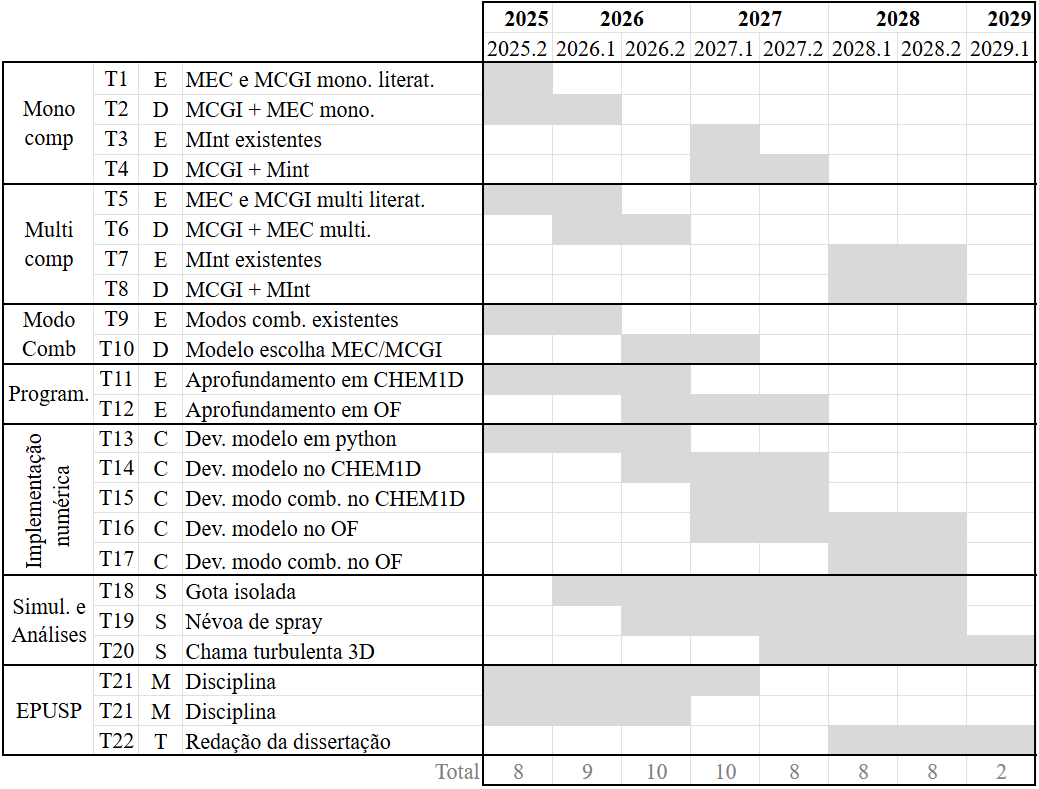
\includegraphics[width=0.9\textwidth]{30_images/cronograma-3.png}
    \label{fig:cronograma}
\end{figure}


Considerando inicialmente gotas monocomponentes, o trabalho proposto se iniciará com o estudo aprofundado sobre MEC e MCGI monocomponentes pré-existentes na literatura (tarefa \textbf{T1}), o que dará base para o desenvolvimento de modelo integral de combustão de gota isolada monocomponente com modelo detalhado de evaporação (tarefa \textbf{T2}).
Em sequência virá o estudo aprofundado de modelos preexistentes para a modelagem analítica de \yellow{de fenômenos de} \yellow{transporte no interior de gota} (tarefa \textbf{T3}), seguido pela avaliação da viabilidade de acoplamento de modelos monocomponente de combustão de gota isolada com discretização no interior da gota (tarefa \textbf{T4}).
A mesma sequência de tarefas procede para gotas multicomponentes, originando as tarefas (\textbf{T5}), (\textbf{T6}), (\textbf{T7}) e (\textbf{T8}). 

Visando utilizar o MCGI desenvolvido em simulações de combustão de spray, faz-se necessário então o estudo aprofundado de modelos de modo de combustão de sprays (\textbf{T9}), focando no modo de combustão de gota isolada e de combustão externa. Em seguida virá o desenvolvimento de um modelo para determinar se a gota utiliza um MEC ou MCGI, baseado nos modelos preexistentes na literatura. (\textbf{T10}).

Para simular os modelos desenvolvidos, é necessário implementá-los no programa a ser utilizado.
Assim, torna-se fundamental o estudo aprofundado dos softwares e das linguagens de programação empregadas. 
No caso da simulação em ambiente simplificado, isso envolve o software CHEM1D e a linguagem Fortran (\textbf{T11}).
Já para a simulação turbulenta multidimensional, envolve o software OpenFOAM e a linguagem C++ (\textbf{T12}).
% Em ambos os casos, o aprofundamento na linguagem de programação visa a implementação do modelo desenvolvido no software utilizado.

Dessa forma, as próximas tarefas abordam a implementação dos MEC e MCGIs desenvolvidos: na linguagem Python  (\textbf{T13}), no  CHEM1D à  (\textbf{T14}) e no OpenFOAM  (\textbf{T16}).
Nos dois últimos, é necessário também implementar o algorítimo de seleção entre MEC e MCGI, originando (\textbf{T15}) e (\textbf{T17}).  
% As tarefas (\textbf{T15}) e (\textbf{T17}) referem-se à implementação do algorítmo do modelo de modo de combustão, que fará a escolha entre MEC e MCGI, nos softwares CHEM1D e OpenFOAM respectivamente.

As primeiras simulações dos modelos desenvolvidos são simulações 0D de evolução temporal de gota isolada em Python (\textbf{T18}). 
Em seguida, vêm as simulações de chama combustão laminar em névoa quiescente de spray no CHEM1D (\textbf{T19}).
Por fim, após aprofundamento em interação chama-turbulência, virão as simulações de chama multidimensional turbulenta no OpenFOAM nas grandes escalas, usando FGM, ATG, e os modelos novos (\textbf{T20}).
As tarefas de simulação detalhadas aqui incluem o pré-processamento, o tempo de simulação e a análise dos resultados (pós-processamento).
As ferramentas utilizadas para a análise dos resultados em cada uma das atividades de simulação são discutidas na Seção \ref{sec:resultados}.

O Programa de Pós-Graduação em Engenharia Mecânica (PPGEM) da EPUSP exige que 9 disciplinas sejam cursadas para doutorado direto.
Elas são representadas pela tarefa (\textbf{T21}).
Algumas disciplinas se destacam devido a sua relevância para o tópico deste projeto \yellow{e foram selecionadas}: Fundamentos de Combustão I (PME5228), Fundamentos de Escoamentos Turbulentos Reativos  (PME5411), Sistemas Particulados (PQI5848), Termodinâmica Avançada I (PME5014), Introdução à Mecânica dos Meios Contínuos (PME5011) e Modelagem de Turbulência para CFD (PME5418).
Demais disciplinas serão definidas ao longo do desenvolvimento deste trabalho.
Por fim, a redação da dissertação é representada pela tarefa (\textbf{T22}).



% \begin{itemize}
% \setlength{\itemsep}{0cm}
% \item[\textbf{T1}] Estudo aprofundado sobre MEC e MCGI monocomponentes pré-existentes na literatura.% Sobre o MEC, estão incluidos o estudo da derivação dos modelos de Abramzon-Sirignano \cite{Sirignano1989}, a formulação de Miller \cite{MillerR1998}, \todo{...}, No que tange a MCGIs, revisitar o modelo de Godsave-Spalding \cite{Law1978,HenningsJ2024MT}, estudar o artigo do Fachini \cite{FachiniF1999}, suas referências e citações, \todo{...} 
% \item[\textbf{T2}] Modelagem analítica de combustão de gota isolada monocomponente com modelo detalhado de evaporação. % Essa tarefa baseia-se na incorporação do modelo de Abramzon-Sirignano \cite{Sirignano1989} ou da formulação de Miller \cite{MillerR1998} no modelo de Godsave-Spalding \cite{Law1978}. %Como todos os modelos citados baseiam-se em soluções analíticas, é visto como provável que 
% \item[\textbf{T3}] Estudo de modelos preexistentes para a modelagem  analítica de discretização do interior de gota monocomponente.% São exemplos de literatura relevante para essa tarefa \source{}.
% \item[\textbf{T4}] Avaliação da viabilidade de acoplamento de modelos monocomponente de combustão de gota isolada com discretização no interior da gota.% Como os modelos de discretização de interior de gota podem envolver soluções numéricas, se será possível desenvolver uma solução analítica para esse problema. Uma solução acoplada numérica-analítica, interna e externamente gota, respectivamente, precisa ser robusta e computacionalmente eficiente para servir em aplicações CFD. 

% \item[\textbf{T5}] Estudo de modelos MEC e MCGI multicomponente preexistentes na literatura.% Exemplos de trabalhos relevantes de MEC multicomponente incluem \source{}.
% \item[\textbf{T6}] Modelagem analítica de combustão de gota isolada multicomponente com modelo avançado de evaporação. % Essa tarefa baseia-se na incorporação dos modelos de Sacomano \cite{SacomanoF2022IJHMT} ou de Wang \source{WangC2012} no modelo de Godsave-Spalding \cite{Law1978}.
% \item[\textbf{T7}] Estudo de modelos preexistentes para a modelagem analítica de discretização do interior de gota multicomponente.% São exemplos de literatura relevante para essa tarefa \source{}
% \item[\textbf{T8}] Avaliação da viabilidade de acoplamento de modelos multicomponente de combustão de gota isolada com discretização no interior da gota. 

% \item[\textbf{T9}] Estudo de modelos de determinação de modos de combustão de gotas de spray, focando no modo de combustão isolada.% São exemplos de literatura relevante para essa tarefa \cite{AggarwalS2014}, \source{}
% \item[\textbf{T10}] Desenvolvimento de modelo analítico para escolha entre MEC e MCGI, baseado na pesquisa do item anterior.

% \item[\textbf{T11}] Aprofundamento em CHEM1D e em Fortran para programação no CHEM1D.
% \item[\textbf{T12}] Aprofundamento em OpenFOAM e em C++ para programação no OpenFOAM.

% \item[\textbf{T13}] Implementação do modelo MEC/MCGI em Python.% para o T18.
% \item[\textbf{T14}] Implementação do modelo MEC/MCGI no CHEM1D.% para o T19.
% \item[\textbf{T15}] Implementação do modelo de modo de combustão no CHEM1D.
% \item[\textbf{T16}] Implementação do modelo MEC/MCGI no OpenFOAM.% para o T20.
% \item[\textbf{T17}] Implementação do modelo de modo de combustão no OF.

% \item[\textbf{T18}] Simulação da evolução temporal 0D de gota isolada em Python.           %, após T15.
% \item[\textbf{T19}] Simulação de combustão laminar de névoa quiescente de spray no CHEM1D. %, após T16.
% \item[\textbf{T20}] Simulação de chama turbulenta 3D nas grandes escalas com FGM e ATF.    %, após T17.

% \item[\textbf{T21}] Disciplinas de pós-graduação.% No programa de Doutorado Direto do PPGEM na POLI-USP, é necessário cursar 9 Disciplinas, cada valendo 8 créditos. Como não é recomendado cursar mais de duas disciplinas por oferencimento, o qual é quadrimestral, as disciplinas serão cursadas ao longo de 5 quadrimestres, aproximadamente 2 anos. Algumas das disciplinas a serem cursadas já foram escolhidas e estão dispostas na Seção \ref{sec:disciplinas}.
% \item[\textbf{T22}] Redação da dissertação.% Estimou-se iniciar a escrita da dissertação nos últimos três semestres.
% \end{itemize}

% !TEX root = ../Proposta.tex

\section{Forma de Análise dos Resultados} \label{sec:resultados}

Diferentes procedimentos serão adotados para a análise dos resultados obtidos em cada etapa de trabalho apresentada na Seção \ref{sec:metod}.
Considerando apenas os resultados numéricos, i.e. das de simulações, os primeiros resultados serão obtidos após o teste do modelo isolado em ambiente Python. 

A simulação da evolução temporal de um modelo de gota, MEC ou MCGI, e a análise desses resultados é uma área que o autor da proposta já tem experiência \cite{HenningsJ2024MT}. 
Nessa análise, são relevantes parâmetros como o tempo de vida da gota, a dependência dos resultados ds condições iniciais da gota e do ambiente e a dependência dos submodelos utilizados, como o de pressão de vapor ou de fração molar de vapor.

No contexto de avaliação isolada de MECs e MCGIs, é de extrema relevância a comparação tanto com resultados experimentais quanto como \yellow{modelos resolvidos}.
Para MECs, considera-se, por exemplo, os trabalhos experimentais \cite{BiroukM2006,PatelU2019,KayaEyiceD2024,ArabkhalajA2024,MaquaC2008}, focados principalmente na influência da turbulência na evaporação.
Para MCGIs, considera-se os trabalhos experimentais na escala da gota \cite{ChoS1990SCI,CandelS1999,ChenG1996CF,Xu2002,BiroukM2000,CuociA2005,SetyawanH2015} e os trabalhos que \yellow{resolvem} o modelo da gota \cite{Stauch2006,CuociA2005,ChoS1990SCI,KazakovA2003CF,MarcheseA1996CF,WangW2024}.

Já nas simulações no CHEM1D, a análise dos resultados se dará baseada na experiência do grupo de pesquisa, assim como na comparação com MECs já desenvolvidos pelo grupo e testados nesse ambiente \cite{SacomanoF2018CTM,SacomanoF2019IJHMT,SacomanoF2021Fluids,SacomanoF2024CF,SacomanoF2025CF}.
Nessas simulações, são relevantes novamente a influência das condições iniciais e ambientais na frente de chama, em particular na velocidade de chama laminar.

Nas simulações multidimensionais, também será valiosa a experiência e os resultados anteriores do grupo de pesquisa \cite{SacomanoF2017CF,SacomanoF2020CF}.
Nessas simulações, é relevante estudar a influência do modo de combustão de gota isolada na estrutura da chama, como proposto nos objetivos do trabalho.